\documentclass[onecolumn, draftclsnofoot,10pt, compsoc]{IEEEtran}
\hbadness=1000 % suppress warnings
\usepackage{graphicx}
\usepackage{url}
\usepackage{setspace}
\usepackage{hyperref}
\usepackage{listings}
\usepackage{cite}
\usepackage{geometry}
\geometry{textheight=9.5in, textwidth=7in}

% 1. Fill in these details
\def \CapstoneTeamName{		Aerolyzer}
\def \CapstoneTeamNumber{		19}
\def \GroupMemberOne{			Daniel Ross}
\def \GroupMemberTwo{			Kin-Ho Lam}
\def \GroupMemberThree{			Logan Wingard}
\def \CapstoneProjectName{		Aerolyzer}
\def \CapstoneSponsorCompany{	NASA JPL}
\def \CapstoneSponsorPerson{		Kim Whitehall}


% 2. Uncomment the appropriate line below so that the document type works
\def \DocType{		%Problem Statement
	%Requirements Document
	%Technology Review
	Design Document
	%Progress Report
}

\newcommand{\NameSigPair}[1]{\par
	\makebox[2.75in][r]{#1} \hfil 	\makebox[3.25in]{\makebox[2.25in]{\hrulefill} \hfill		\makebox[.75in]{\hrulefill}}
	\par\vspace{-12pt} \textit{\tiny\noindent
		\makebox[2.75in]{} \hfil		\makebox[3.25in]{\makebox[2.25in][r]{Signature} \hfill	\makebox[.75in][r]{Date}}}}
% 3. If the document is not to be signed, uncomment the RENEWcommand below
\renewcommand{\NameSigPair}[1]{#1}

%%%%%%%%%%%%%%%%%%%%%%%%%%%%%%%%%%%%%%%
\graphicspath{{images/}}
\begin{document}
	\begin{titlepage}
		\pagenumbering{gobble}
		\begin{singlespace}
			
\includegraphics[height=4cm]{coe_v_spot1}
			\hfill 
			% 4. If you have a logo, use this includegraphics command to put it on the coversheet.
			%\includegraphics[height=4cm]{CompanyLogo}   
			\par\vspace{.2in}
			\centering
			\scshape{
				\huge CS Capstone \DocType \par
				{\large\today}\par
				\vspace{.5in}
				\textbf{\Huge\CapstoneProjectName}\par
				\vfill
				{\large Prepared for}\par
				\Huge \CapstoneSponsorCompany\par
				\vspace{5pt}
				{\Large\NameSigPair{\CapstoneSponsorPerson}\par}
				{\large Prepared by }\par
				Group\CapstoneTeamNumber\par
				% 5. comment out the line below this one if you do not wish to name your team
				\CapstoneTeamName\par 
				\vspace{5pt}
				{\large
					\NameSigPair{\GroupMemberOne}\par
					\NameSigPair{\GroupMemberTwo}\par
					\NameSigPair{\GroupMemberThree}\par
				}
				\vspace{20pt}
			}
			\begin{abstract}  
				The Aerolyzer Project aims to deliver a new source of air quality and weather information through leveraging existing weather data and image analysis algorithms.
				% characterize aerosol content in the atmosphere
				When complete, this open-source project shall feature a Python library that uses image classification and third-party weather APIs, displayed with an intuitive web-based user interface.
				This document outlines the software design descriptions for the Aerolyzer Library. 
			\end{abstract}     
		\end{singlespace}
	\end{titlepage}

\section{Table of Contents}
\tableofcontents
\clearpage

\begin{singlespace}
\section{Overview}
	\subsection{Scope}
		Aerolyzer mobile web application is intended to retrieve data from user images in order to analyze colors in the images using wunderground data and image analysis software. This application proposed by NASA JPL is intended for aiding in the scientific research of air quality and of aerosols in the atmosphere. 
	\subsection{Purpose}
		This document describes the three main components of Aerolyzer that will be designed, those being the library data interface, the horizon detection filter and the library structure. 
	\subsection{Intended Audience}
		The intended audience for this software design document is the Aerolyzer developers and clients. It will serve to set design intentions so that the client can confirm the design plan will meet the requirements.

\section{Definitions}
	
	\subsection{Aerosol}\label{def:aerosol}
		Aerosols are tiny particles dispersed throughout the atmosphere.
		These particles originate from natural sources such as volcanic eruptions, and unnatural sources such as pollution. 
		One can visibly see the effects of aerosols in the 'Rayleigh scattering effect'  which visibly reddens sunsets and sunrises. \cite{allen_2015}
	
	\subsection{Acceptable Image}\label{def:accImg}
		An acceptable image is defined as an unedited image of the horizon. \ref{def:horizon}
		Images used in data collection must have valid EXIF meta data, while the images used in training classifiers only require relevant image content. \ref{def:exif}
	
	\subsection{Horizon}\label{def:horizon}
		The horizon is defined as the line at which the sky and earth's surface appear to meet.
	
	\subsection{EXIF}\label{def:exif}
		Exchangeable image file format.
	
	\subsection{Local}\label{def:local}
		Local is defined as the circular area around an observer with the radius being the distance from an observer's position to the horizon.
		For an observer on the ground, this distance is approximately 2.9 miles (4.7 km) and for an observer standing at an elevation of 100 ft (30 m) above ground level this distance is approximately 12.2 miles (19.6 km).

\section{Design Description Information Content}
	\subsection{Introduction}
    
    \subsection{Software Design Description Identification}
    	\subsubsection{Library Data Interfaces}
        The Aerolyzer Python library will need to have a framework to receive input from the user, send the results of the functions to the HTML which will display them, store data for later use, and retrieve data relevant to a user’s request.
        \subsubsection{Horizon Detection Filter}
        The Aerolyzer library hopes to feature a module that infers aerosol size based on the hue distribution in images of the sunrise or sunset. To this end, a filter that intelligently recognizes acceptable images \ref{acc_img} is necessary to save computation time and guarantee reliable data.
        \subsubsection{Library Structure}
        The Aerolyzer library aims to be accessible to import for scientific research purposes. The structure of this library will determine the ease of access of this library.
	\subsection{Identified design stakeholders}
    	\subsubsection{Library Data Interfaces}
        The stakeholder in the Library data interfaces will be the users submitting ZIP codes and images. Without the proper channels for data transfer, the user’s will never receive results from the library and the library will never receive requests from the users.
        \subsubsection{Horizon Detection Filter}
        The stakeholders for the Horizon Detection Filter python module include users who will be using the Aerolyzer web service. Users will ideally not have to wait for long periods of time for the server to process weather and air quality analysis. The horizon filter will expedite this process by filtering out bad data.
        \subsubsection{Library Structure}
        The stakeholders for the Aerolyzer library’s structure will be the developers and the Aerolyzer’s primary stakeholder, Dr. Kim Whitehall. The Dr. Whitehall requires the library to be accessible from Python’s package index.
\section{Selected Design Viewpoints}
	\subsection{Library Data Interfaces}
      \subsubsection{Design Elements}
          \paragraph{Design Attributes}
          Django is the python based web framework hosting the Aerolyzer application\cite{DjangoStart}.
          The purpose of using Django is to enable servers to present the input prompts to the user and then present the output of the Python Library to the user.
          The Django framework works on models that map out the database that the application is stored on \cite{DjangoDoc}.
          Django is open source and written by Django Software Foundation \cite{DjangoOver}.
		  
          The Python library functions will be called by HTML code reacting to the user input.
		  Once the library functions\ref{des:LibStructure} receive the user input, the library will store the user’s input and data associated with it in the database.
		  The results returned from the library calls to the html code will coincide to a change in web page that will display returned data using Google Charts \cite{GoogleCh}.
          \paragraph{Design Relationships}
            \begin{figure}[h]
            	\centering
                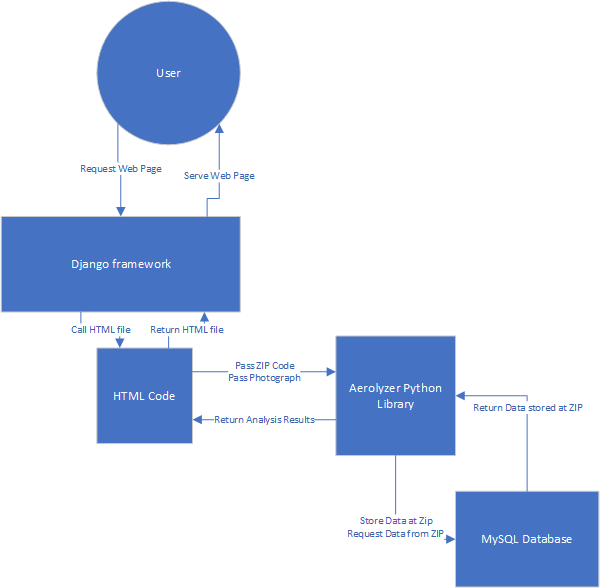
\includegraphics[width=4.5in]{DesignInterface}
                \caption{Library Interfaces}
                \label{fig:1}
            \end{figure}
          \paragraph{Design Constraints}
          The Python Library functions must make their calls to the MySQL database discrete in order to maintain consistent data between multiple users.
          The HTML code of the application has to handle each page request correctly and pass any input from the user to its requests sent to the Aerolyzer library. 
          Additionally, Google Charts is a imported javascript resource which will require a consistent internet connection when Django starts processing the web page.
      \subsubsection{Design overlays}
      Django will provide the data models for user input and the library output.
      These models will be an Image class, for all cases where an user submits an image, and a ZIP class, for all cases where an user submits a ZIP code in lieu of an image.
	  Each class contains all of the fields for the data that the HTML will need in either case. This will contain weather API data, results, and user data in both cases.
	  EXIF field, Image ID field, and filename are unique to the Image class while the ZIP field is unique to the ZIP class. 
		\begin{lstlisting}[language=Python]
        from django.db import models
        
        class Image(models.Model):
            imageId = models.AutoField(primary_key=True)
            filename = models.CharField(max_length=200, default = "none")
            exif = models.CharField(max_length=200)
            wunder = models.CharField(max_length=200)
            results = models.CharField(max_length=200)
            
        def __unicode__(self):
            return self.results
			\end{lstlisting}
            The HTML code will call on the Google Charts API on the results display page which Django will only navigate to if there were no issues for the Library.
			In the case that the user inputs an invalid ZIP code, rather than attempt to navigate to a new page the HTML code will display an error.
			Django’s input forms will designate what types of files are accepted for image upload and an error message will be thrown if the image isn’t a .png, .jpeg, or .jpg.
			
			The MySQL database will use ZIP codes as primary keys which subsequent weather data, image analysis, and images will be stored under.
      
      \subsubsection{Design rationale}
		Using the Django framework serves as a reliable and appealing option for multiple reasons. Django, like the Aerolyzer library, is written in Python so the resulting interfaces with any HTML code is going to be written in python which offers additional consistency to development. Django’s built in templating API and development tools also remove the need for additional imported software that some other frameworks require.\cite{DjangoStart}\cite{DjangoOver}
			Setting the Aerolyzer library in between the front end of the web framework and the back end of the MySQL database is the design choice here, because the Library’s functions are the only component that need to read or write to the database.
     
      \subsubsection{Design languages}
		As stated previously, Django is written in python \cite{DjangoOver}. The web pages will be written in HTML5 and utilize javascript in order to use Google Charts \cite{GoogleCh}. The MySQL database is used with SQL (Structured Query Language).

	\subsection{Horizon Detection Filter}
      \subsubsection{Design Elements - OpenCV & Google Tensorflow}
      		\paragraph{Design Attributes}
          		Outlined in the Software Design Document, a horizon detection filter shall be created using OpenCV and other python libraries as required. OpenCV is a BSD-licensed computer-vision library with many relevant sub-modules. Containing over 2,500 algorithms, OpenCV can analyze images and videos, recognize faces, identify objects, perform visual transformations, and more. One can use image transformations to normalize image data such that a classifier can more easily distinguish what is in a given image. 

				An advanced machine learning library, Google Tensorflow can build versatile and accurate predictive data models provided a large dataset of training images. One can apply Tensorflow to the Aerolyzer project by training its inception module to recognize patterns in a large dataset consisting of acceptable images of the horizon. A human will need manually pre-classify and build a test dataset consisting of acceptable images. \ref{acc_img}  Tensorflow’s ease of use, proven library, and ample documentation makes it a potential candidate to create a powerful image classifier.

				As of December 2017, Kin-Ho Lam has designed and tested two horizon detection classifiers using OpenCV 3.3.0. Ongoing work on the project can be viewed in the Aerolyzer library’s open-source Github. \cite{OUR GITHUB} These classifiers are horizon detection by straight line and horizon detection by color threshold.

          \paragraph{Design Relationships}
          		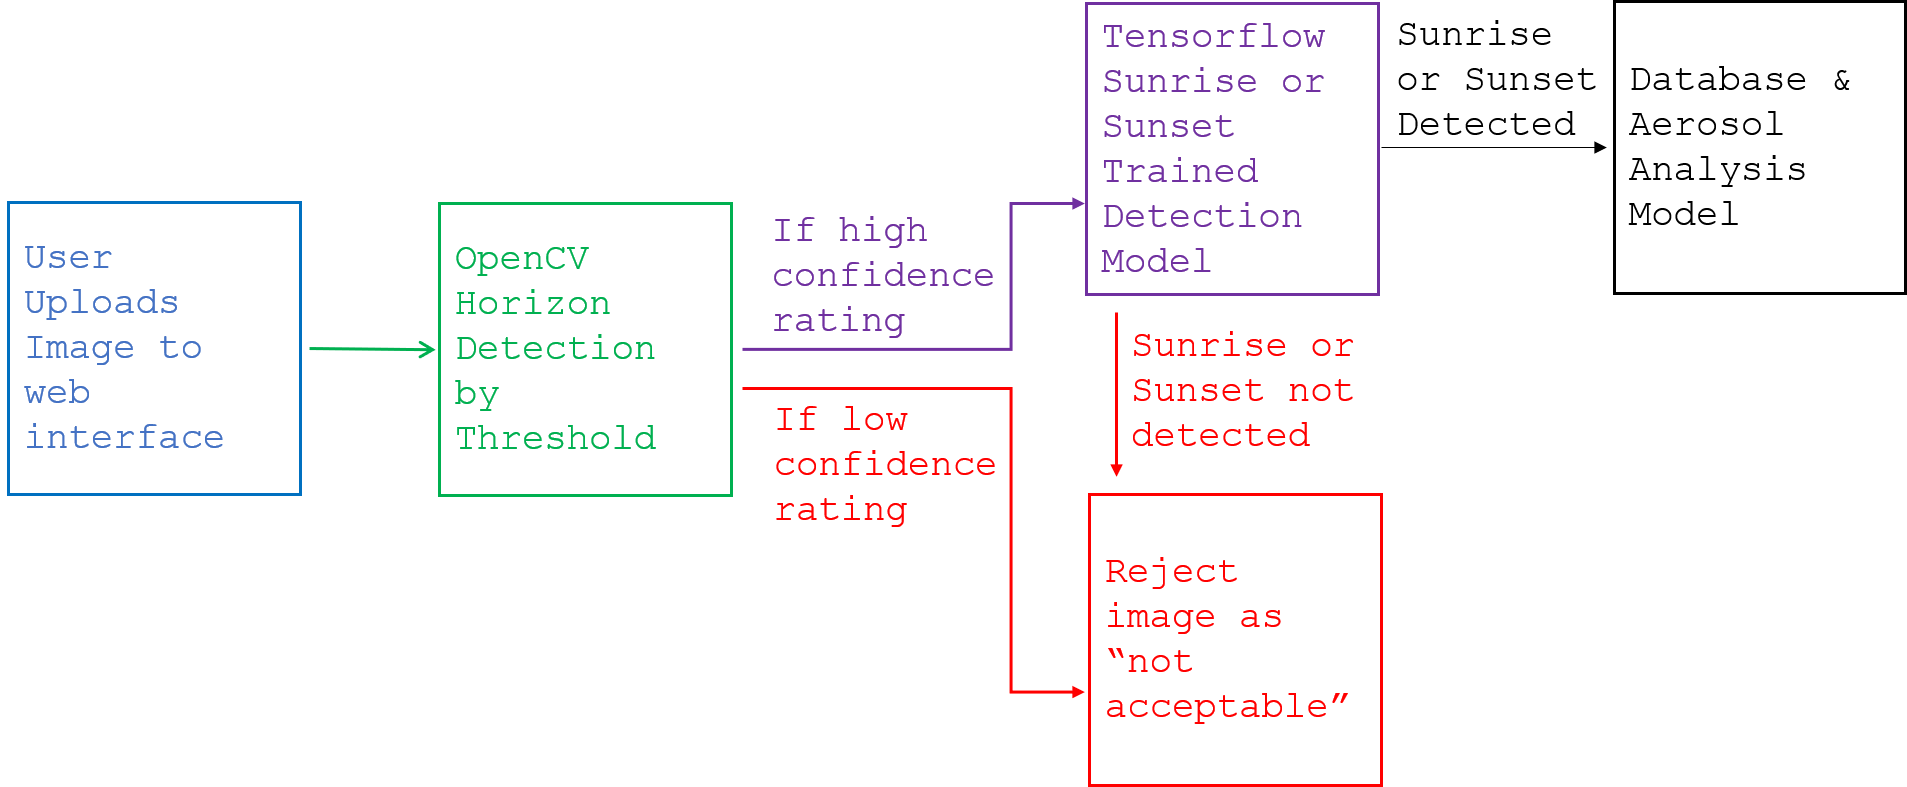
\includegraphics[width=4.5in]{tensor}

          \paragraph{Design Constraints}
          		Aerolyzer’s unique image criterion necessitates a predictive data model capable of detecting horizons with a minimum of 66\% certainty and sunsets or sunrises with a minimum of 50\% certainty. Efficient and expedient algorithm performance is necessary due to the expected user base who will be waiting for Aerolyzer to service their request. Pending further research, these criterion are achievable through OpenCV and Tensorflow. More computer vision libraries or modules may be required.
      
      \subsubsection{Design overlays}
      		\paragraph{OpenCV Horizon Detection by Straight Line Algorithm}
      			Horizon detection by straight line seeks to detect the simplest possible acceptable image; a picture of the sunset/sunrise without obstructions. In this case, one can expect the most visible longest and straightest line in an image to be the horizon. With this assumption, the Horizon Detection by Straight Line algorithm shall accept or reject an image through the following procedure:
      			\begin{enumerate}
      				\item Upon receiving an image, detect the longest and straightest line.
      				\item If there is no straight line stretching across the image, reject it.
      			\end{enumerate}
      			As a proof of concept, the algorithm is implemented in the following python function. This algorithm draws a straight green line where it believes the horizon is.
      			\lstinputlisting[language=Python]{code/HorizonDetectionbyStraightLine.py}
     			
     			Upon being fed an image, the Horizon Detection by Straight Line’s algorithm works as follows:
				

				\begin{enumerate}
					\item Perform a gaussian blur on the image
					\item Convert the image to grayscale
					\item Perform Canny Edge Detection \cite{canny_edge}
					\item Perform Hough Line Transformation \cite{houghLines}
					\item If there is a straight line, draw a green line spanning across the image. This is the classified horizon.
					\item Else, if there are no straight lines, then reject the image.
				\end{enumerate}


				This approach works well for some images such as fig X pulled from the Aerolyzer test image album. However, it is clear that this approach does not work for all cases, as seen in fig Y, detecting the horizon by straight line fails in images with a complex foreground that contains many straight lines. A new algorithm is necessary to enhance detection accuracy.

				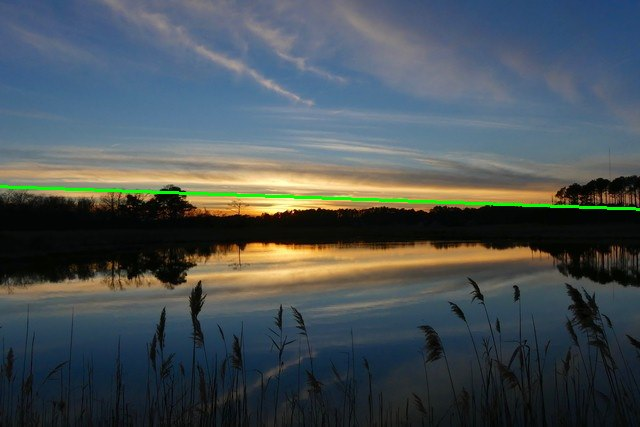
\includegraphics[width=4.5in]{line1}
				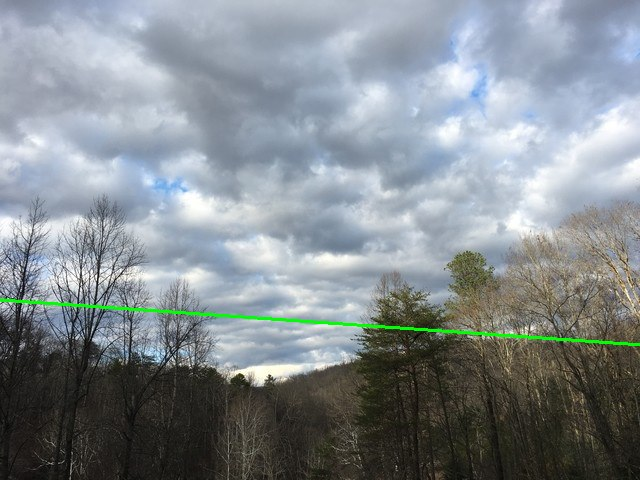
\includegraphics[width=4.5in]{line2}

				\paragraph{OpenCV Horizon Detection by Threshold}
					Horizon Detection by Threshold is a more versatile method compared to straight line detection because it relies on segmenting color distribution. Detection by Threshold was designed to classify images that contain complex foregrounds by distinguishing what part of the image is the sky. The Threshold algorithm shall accept or reject an image through the following procedure:
					\begin{enumerate}
						\item Separate the image by distinct color spaces
						\item Perform a binary threshold with the minimum color threshold being the color of the sky.
						\item Calculate the area of the largest continuous contour that is within the sky color threshold.
						\item Apply a statistical function to ratio the area of sky color over the total area of the image to produce a confidence rating. A high confidence rating shall indicate that the image contains a horizon while a low confidence rating indicates there is no horizon.
					\end{enumerate}

					As a proof of concept, the algorithm is implemented in the following python function. This algorithm draws a green outline of what it believes to be the sky.

					\lstinputlisting[language=Python]{code/HorizonDetectionbyStraightLine.py}

					Upon being fed an image, (this example features Fig. Y) the Horizon Detection by Threshold works as follows:
					\begin{enumerate}
						\item Convert image into converted to TCbCr digital color space (not to be confused with YUV colorspace).
							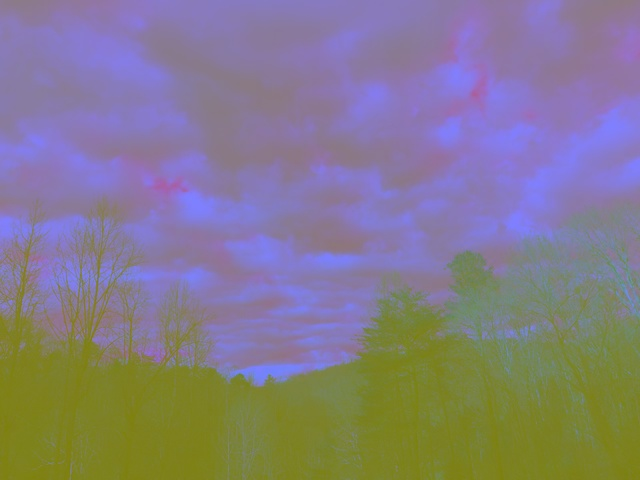
\includegraphics[width=4.5in]{threshold/1}
						\item A TCbCr digital color space separates the pictures intensity from its colors, enabling a histogram equalization on the blue channel. After performing this equalization, the red-green-blue channels are merged back together. This enables a separation of the sky and clouds from the foreground.
							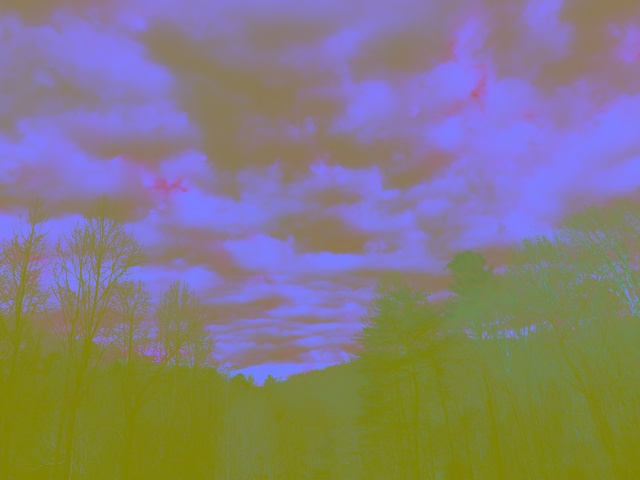
\includegraphics[width=4.5in]{threshold/2}
						\item This separation of sky and foreground becomes clearer after the image is converted back to BGR.
							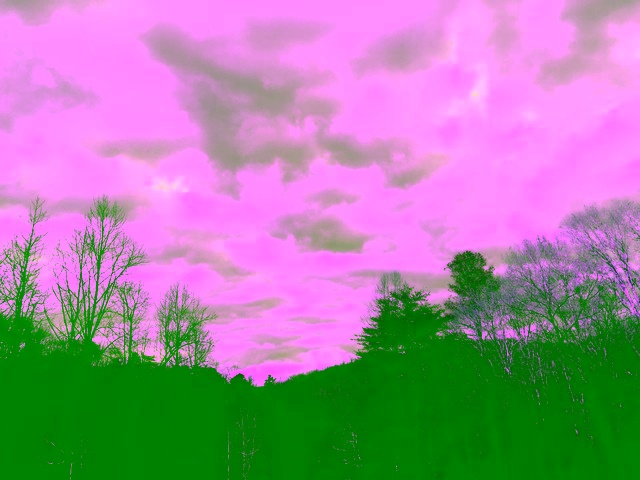
\includegraphics[width=4.5in]{threshold/3}
						\item Prepare to segment the sky from the foreground by greyscaling the image and applying a gaussian blur.
							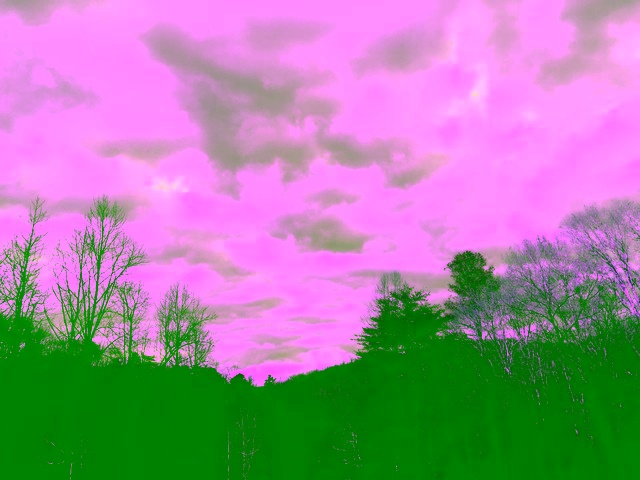
\includegraphics[width=4.5in]{threshold/3}
						\item Apply a binary threshold; if a pixel value is at least 120, it is assigned grey otherwise it is assigned a black value.
							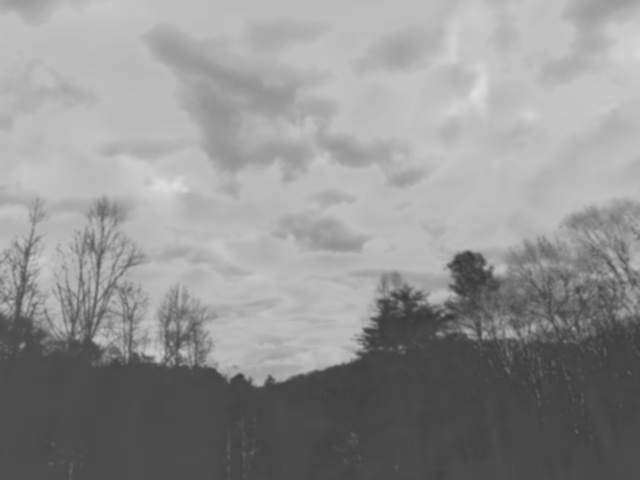
\includegraphics[width=4.5in]{threshold/4}
						\item Erode the image to de-noise and improve clarity.
							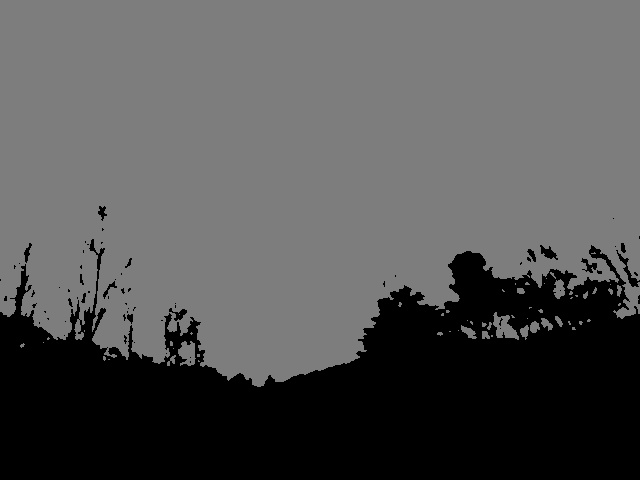
\includegraphics[width=4.5in]{threshold/5}
						\item Finish de-noise with a dialite to de-chunk the image.
							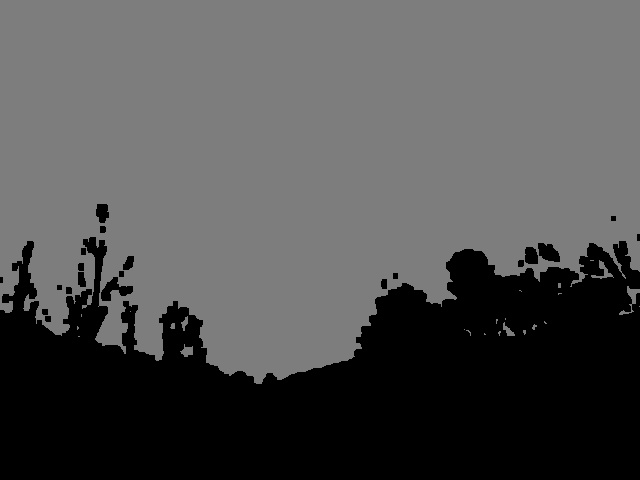
\includegraphics[width=4.5in]{threshold/6}
						\item Draw contours, in this case it visually appears as a white outline around the largest continuous grey section.
							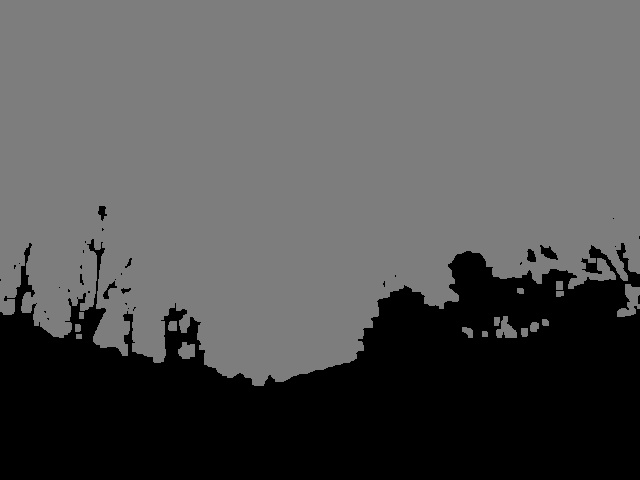
\includegraphics[width=4.5in]{threshold/7}
						\item If contours can be drawn, then the largest contour is overlaid on the original image. Fig. Y “passes” as acceptable and as see it accurately outlines the visible sky.
							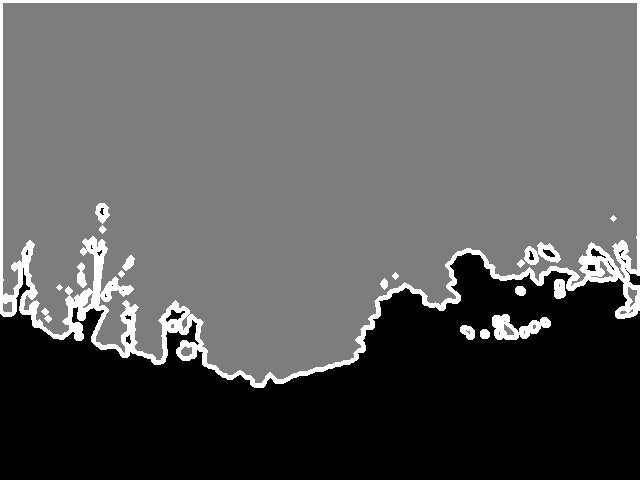
\includegraphics[width=4.5in]{threshold/8}
						\item If no contours can be drawn, the algorithm fails the image, meaning no sky or horizon can be detected.
							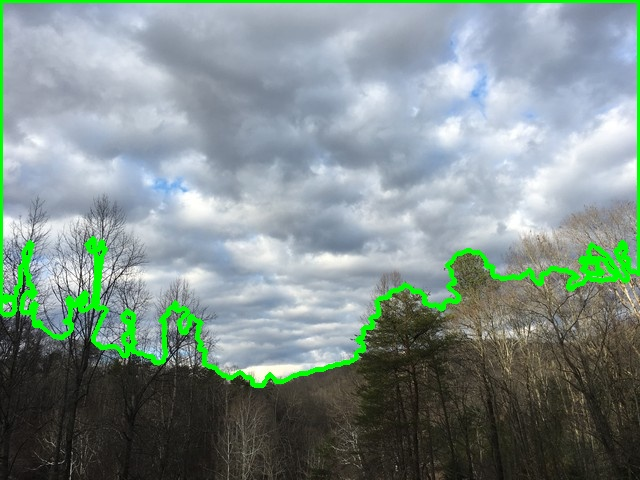
\includegraphics[width=4.5in]{threshold/9}
					\end{enumerate}
					This algorithm struggles to classify low-light images, improvements and fine-tuning are necessary. One can see the threshold algorithm works well for fig. Y.

      \subsubsection{Design Rationale}
      	The Aerolyzer Horizon Detection Filter needs to identify acceptable images, namely ones of the sunset or sunrise. Research indicates that specific sunset or sunrise image classification  necessitates a predictive Tensorflow model because creating such an unsupervised classifier in OpenCV is a challenging task. As demonstrated in Fig. Z, this design rationale is accomplished by incorporating a trained Tensorflow model as a secondary step after OpenCV Horizon Detection by Threshold. Tensorflow analysis is a computationally expensive process. An OpenCV classifier to detect the presence of the sky saves computation time by rejecting all images that do not have skies. If no sky is present then it logically follows that there can be no sunrise or sunset in the image.

      \subsubsection{Design languages}
      	An element in the greater Aerolizer python library, the horizon detection algorithm shall be written in Python 2.7.12 while importing OpenCV 3.3.0 and Numpy 1.13.3. The Aerolyzer project’s sponsor, Dr. Whitehall, chose Python as the library’s primary language. 

	\subsection{Library Structure}\label{des:LibStructure}
      \subsubsection{Design Elements}
          \paragraph{Design Attributes}
                    One goal of Aerolyzer is to create an accessible python package capable of being imported and giving access to all of the horizon detecting and color analyzing software written when creating a functioning Aerolyzer mobile web application. This will include an Apache licensed python script setup.py that ensures required packages such as numpy 1.8.0, exifread, opencv-python, and pyyaml are installed. 
      The structure of this library is important to the usability of the library. To maximize simplicity and usability of the Aerolyzer library, the semantics of the python init file need to make it clear where each function is from. Aerolyzer is designed such that “import aerolyzer” will be the needed import to access the aerolyzer functions later on in the code by calling “aerolyzer.<function-name>()”.
			In the Aerolyzer package, \_\_init\_\_.py is a python file that determines how a module is imported. Aerolyzer’s \_\_init\_\_.py contains imports of the python scripts that supply Aerolyzer functionality. Setup.py is a python file that determines which packages will be installed when downloading the Aerolyzer module. The code for these files can be seen here.
            \_\_init\_\_.py
            \begin{lstlisting}[language=Python]
            version = "0.0.0.4"
            import image_restriction_functions
            import image_restriction_main
            import retrieve_image_data
            from wunderData import *
            from horizon import *
			\end{lstlisting}
            setup.py (The line that sets the required packages)
            \begin{lstlisting}[language=Python]

            _requirements = ['exifread', 'numpy>=1.8.0', 'opencv-python', 'pyyaml',]

            \end{lstlisting}
          \paragraph{Design Relationships}
          When importing Aerolyzer, the \_\_init\_\_.py script executes and imports all python scripts with Aerolyzer functionality, including wunderground data script, image restriction script, image analysis script, etc.
          \paragraph{Design Constraints}
          The setup script for importing Aerolyzer is licensed under the Apache License, Version 2.0 and is constrained to the compliance of said licence. 
      \subsubsection{Design overlays}
      		The Aerolyzer library is Under the Apache Licence Version 2.0 and follows Apaches permissions and limitations.
      \subsubsection{Design rationale}
      		The choice to use python’s package index is to keep the Aerolyzer library open source enabling software developers, data analysts, etc. to access the Aerolyzer library and use its image analyzing software for their own research needs. 
      \subsubsection{Design languages}
      The language used will be python 2.7.12 to write a setup script for when importing Aerolyzer.




\section{Bibliography}
	\bibliographystyle{IEEEtran}
	\bibliography{ref}

\end{singlespace}
\end{document}
